\chapter{Distance Sampling\label{sec:dist_comp}}



\begin{enumerate}

\item \textbf{Line transect estimation from the a minke whale survey}: The survey from which these data were obtained is described in Branch, T.A. and D.S. Butterworth (2001) Southern Hemisphere minke whales: standardised abundance estimates from the 1978/79 to 1997/98 IDCR-SOWER surveys. Journal of Cetacean Research and Management 3(2): 143-174, which is on MMS. The survey region is shown in Figure 1(e) on page 146 of that paper.

\begin{enumerate}

\item \textbf{Getting started}: Open \texttt{RStudio} and in it open a new \texttt{R script} window (using the button top left). Load the \texttt{R} package \texttt{Distance} by typing 

\verb|library(Distance)|

in the \texttt{R script} window and then clicking on the 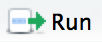
\includegraphics[scale=0.7]{Run.png} button with your cursor on the line that you just entered. Now do the same for the command

\verb|data(minke)|

which loads a minke whale survey dataset. You can find out a bit about it by typing 

\verb|?minke|

which opens the \texttt{minke} help pages in \texttt{RStudio}'s Help window. 

Have a look at the data by typing \verb|head(minke)| or clicking on \verb|minke| in the top right window (Figure~\ref{fig:RStudio}).

Plot a histogram of the observed perpendicular distances (\verb|minke$distance|) using the \verb|histogram| command.

\item \textbf{Fitting a model}: Typing

\verb|?Distance|

opens the \texttt{Distance} help pages in \texttt{RStudio}'s Help window. Click on the ``Index'' link at the bottom of this page and browse the topics. Look in particular at the \verb|ds| command. (You should be looking at something like Figure~\ref{fig:RStudio}.)

\begin{figure}[h!]
\caption{RStudio window.}
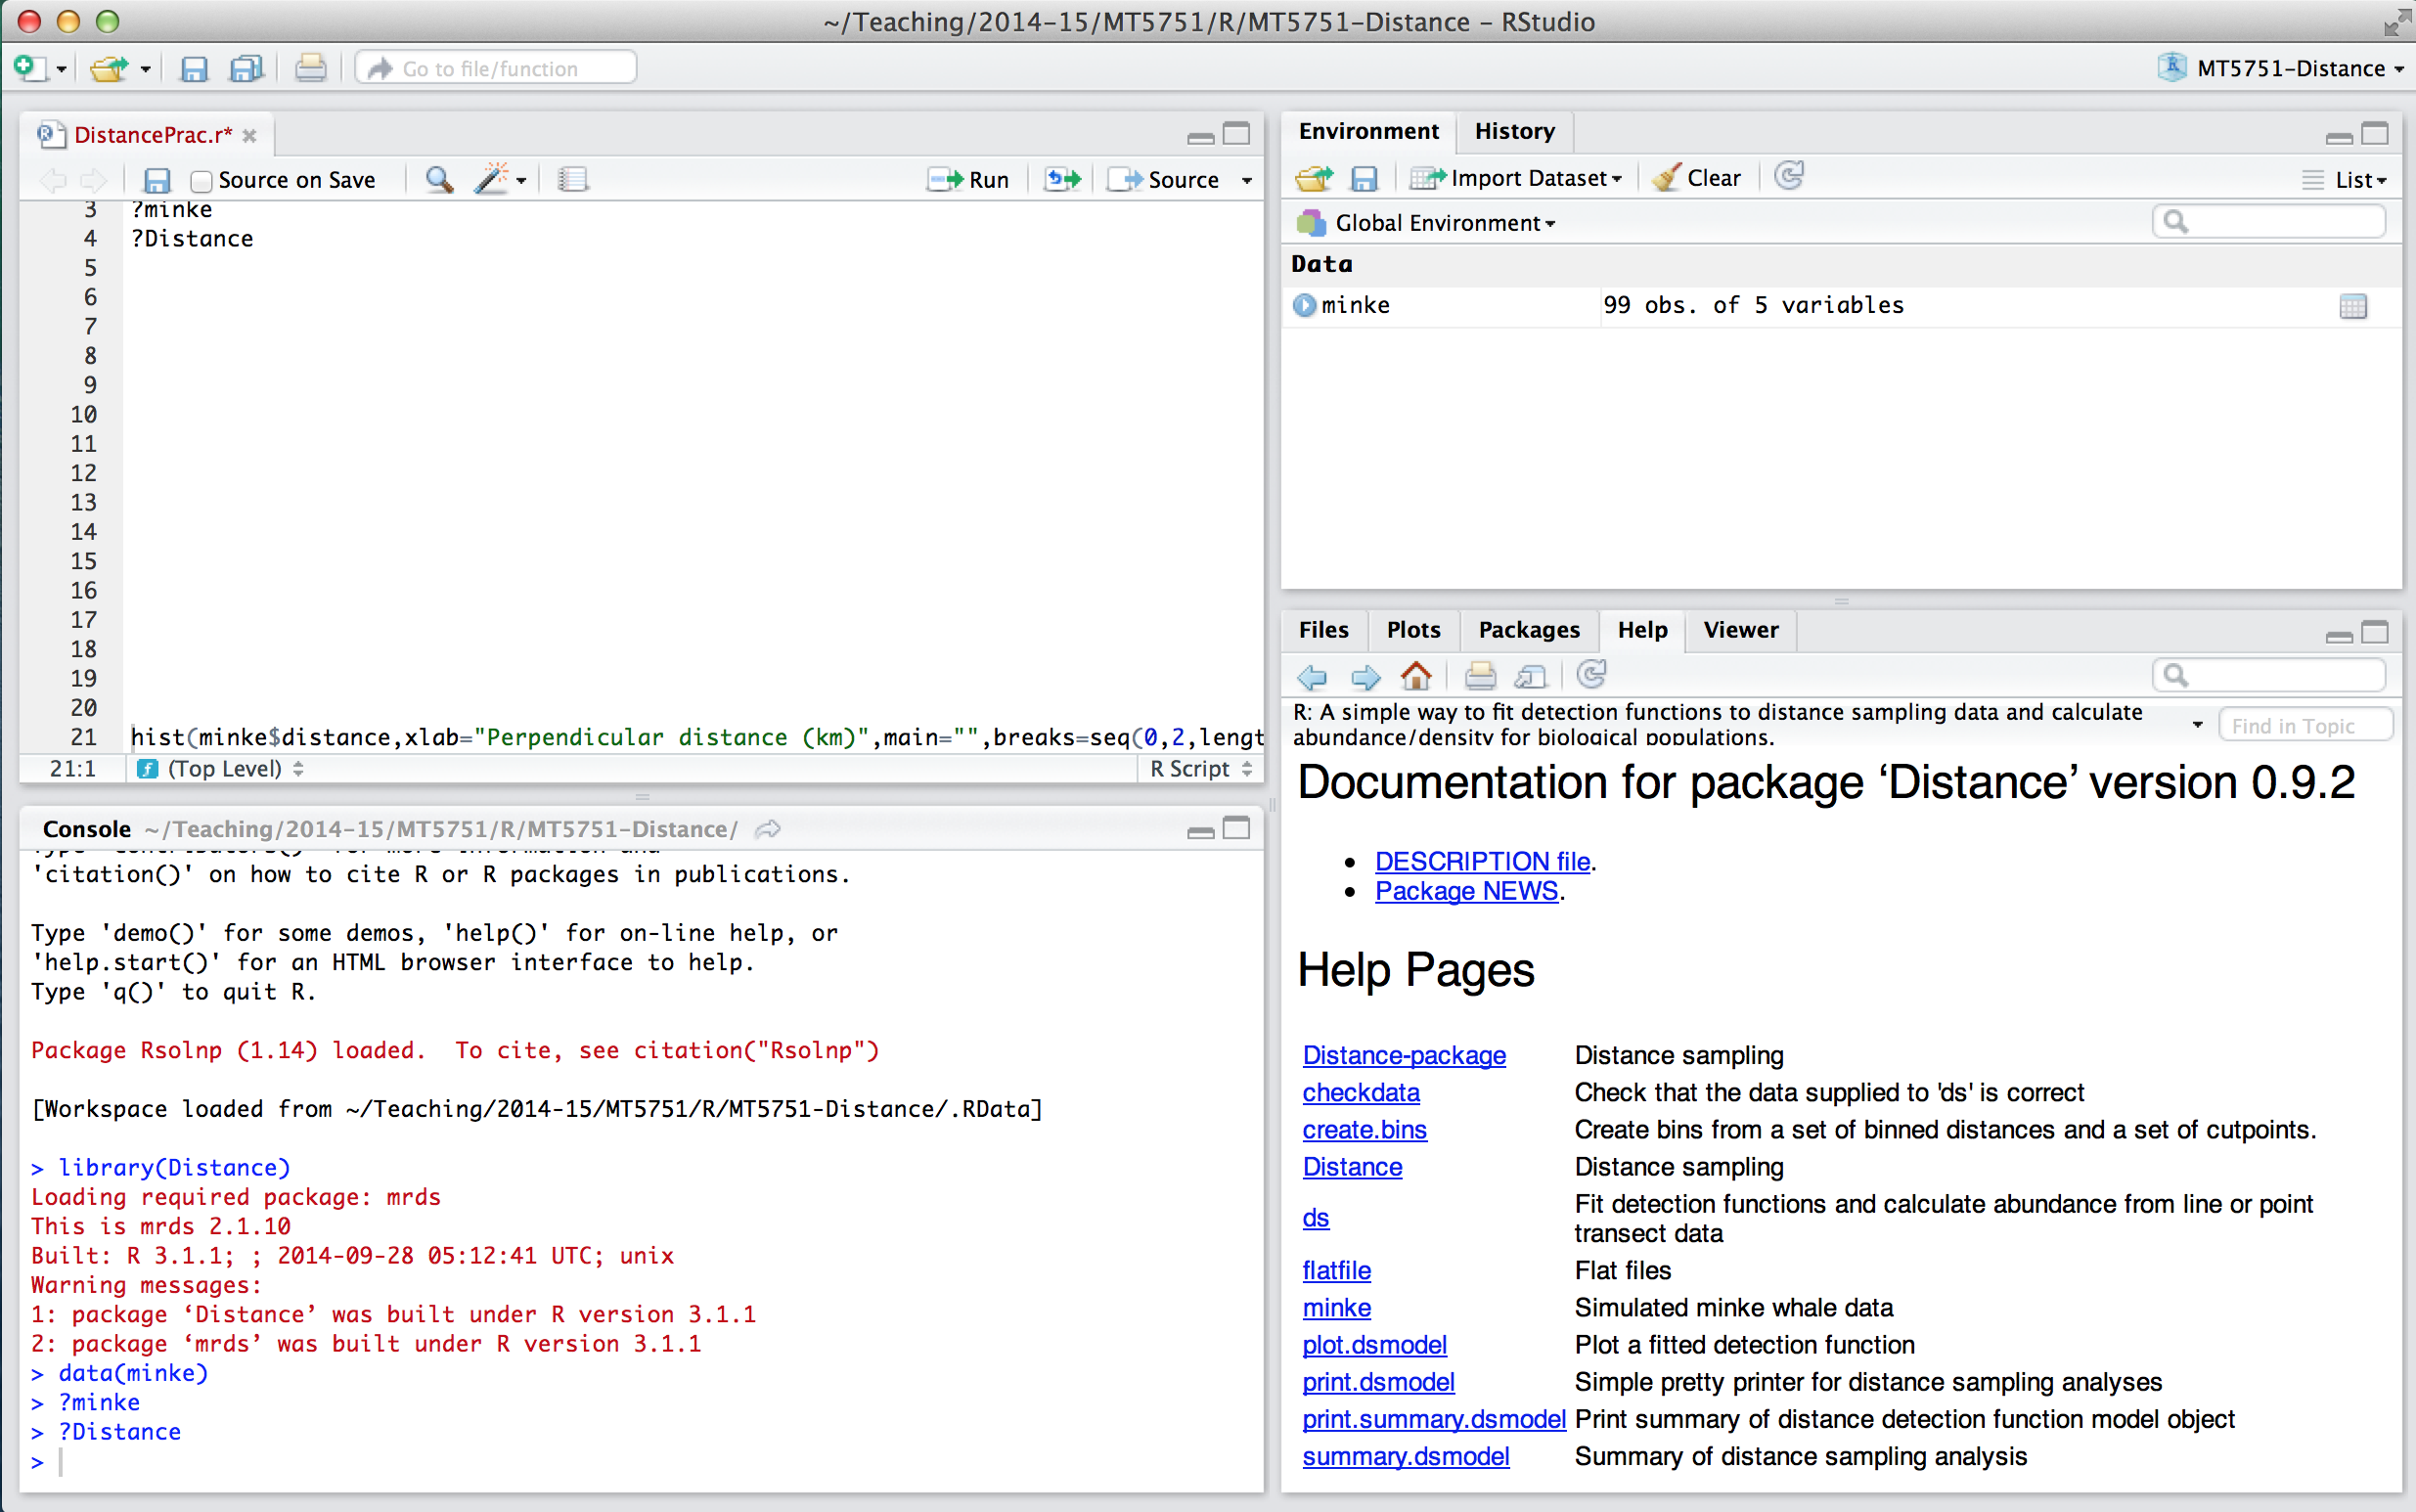
\includegraphics[width=14cm]{RStudio2.png}
\label{fig:RStudio}
\end{figure}

Use the function \verb|ds| to fit a half-normal detection function model and estimate the number of minke whales in the area covered by this survey. 

Having fitted a model with the command \verb|ds|, you can look at the estimates using the \verb|summary| command. (For example, if your fitted model is in an object called \verb|fit.hn|, type \verb|summary(fit.hn)| to look at the estimates obtained in fitting.)

Note that in order to keep them positive, detection function scale parameters are parameterised as $\sigma=\exp(\beta)$ in the package \verb|Distance|, and it is the estimate of $\beta$, not $\sigma^2$ that \verb|summary| reports. Using this fact, verify that $\hat{\sigma}^2$ is about 0.495

\item \textbf{Find the best estimate}: Now try more than one detection function form, select a model using some statistically valid criterion, and check goodness-of-fit of the model, using the function \verb|ddf.gof|. You can get the help page for \verb|ddf.gof| by typing \verb|?ddf.gof|. \textit{Note: You will need to pass the} \verb|$ddf| \textit{component of the object returned by} \verb|ds| \textit{into} \verb|ddf.gof| \textit{-- if you pass the whole object it will not work. (This is a bug in that is currently being addressed.)}

\end{enumerate}

\end{enumerate}
